\subsection{Matrix Methods}
In this section, we consider methods that construct Euclidean embeddings by approximating matrices. In order to make sense of graph data, we consider matrices that encode the structural properties of the underlying network. In Section \ref{MDS} we describe a method to embed graphs into Euclidean space starting from its shortest path matrix, while in Section \ref{Spectral-Emb} the matrix in question will be the normalized Laplacian matrix of the graph.

\subsubsection{Multidimensional Scaling (MDS)}\label{MDS}
Multidimensional Scaling (MDS) (\cite{kruskal1964multidimensional}) (see also \cite{cox2000multidimensional} and \cite{borg2003modern}) is a method for creating a Euclidean embedding of data for which one has information about distance or dissimilarity among the datapoints. For instance, given an $N \times N$ matrix of distances between $N$ points, one can embed the points into $\mathbb{R}^k$, so as to preserve distance information. In particular, one can use MDS as a way to create useful features for graphs by considering the shortest path distance between vertices. MDS is similar to PCA, except instead of using correlation information, we make use of pointwise distances.

Classical Multidimensional Scaling works as follows: let $D$ be the dissimilarity matrix. Then:
\begin{enumerate}
  \item Let $D^{(2)}$ be the point-wise square of the distance matrix,
  \item Let $J = I - {1\over n}{\mathbf{1}}{\mathbf{1}}^T$,
  \item Let $B = -{1 \over 2}JD^{(2)}J$,
  \item Find the top $m$ eigenvalues of $B$ $\lambda_1, ... \lambda_m$, and the corresponding eigenvectors $e_1, ... , e_m$,
  \item Let $X = E_m\Lambda^{1/2}$.
\end{enumerate}

Classical Multidimensional Scaling minimizes a loss function called \emph{strain}:
\[
    \text{Strain}_D(x_1, ... , x_N) = \left( ({\sum_{i,j}b_{i,j}- \langle x_i,x_j \rangle})^2 \over \sum_{i,j}b_{i,j}^2\right).
\]

Classical MDS only works for Euclidean spaces, so in the context of graphs, where the underlying metric is given by shortest path metric, we use a slightly different version of MDS. This variant, known as metric MDS, finds en embedding $x_1, ... , x_n$ minimizing the following objective function (stress):
\[
    \text{Stress}_D(x_1, ... , x_n) = \left(\sum_{i < j = 1, ... ,N}(d_{ij} - ||x_i - x_j||)^2\right)^{1/2}
\]

This minimization is done through the SMaCoF (scaling by majorization for complicated functions) algorithm (\cite{de2011applications}). Note that the stress can be written as:

\[
  \text{Stress}_D(x_1, ... , x_n) = \sum_{i < j} d_{i,j}^2 - 2\sum_{i<j} d_{i,j}||x_i - x_j|| + \sum_{i<j} ||x_i - x_j||^2
\]
where the first summand is a constant:
\[
    C = \sum_{i < j} d_{i,j}^2
\]
the second term is quadratic in $X$: it equals $X^THX$ where $H$ is the hessian matrix, and the third term is bounded by:
\[
    \sum_{i<j} ||x_i - x_j||^2 \geq \text{tr}(X^TB(Z)Z)
\]
where:
\[
    B(Z)_{i,j} = \begin{cases} {d_{i,j}\over||z_i - z_j||} &\text{if }||z_i - z_j||\neq 0 \text{ and }i\neq j\\
    \hspace{5mm}0 &\text{if } ||z_i - z_j|| = 0\text{ and }i \neq j\\
    -\sum_{k \neq i}B(Z)_{i,k} &\text{if } i=j\end{cases}
\]
Where $Z$ is given in the following algorithm:

\begin{algorithm}[H]
\SetAlgoLined
\While{$\sigma(X^{k-1})  - \sigma(X^{k}) \geq \epsilon$}{
  $Z \gets X^{k-1}$ \\
  $X^k \gets \underset{X}{\min}\hspace{1mm} \tau (X,Z)$
}
\caption{SMaCoF algorithm}
\end{algorithm}

where:
\[
  \tau(X,Z) := \sum_{i,j}d_{i,j}^2 + \text{tr}(X^T V X) - 2 \text{tr}(X^TB(Z)Z)
\]
MDS on Graphs is also used as the core component of Isomap, a popular method for manifold learning.

\subsubsection{Spectral Embedding}\label{Spectral-Emb}
Another way to embed a graph in Euclidean space is given by the spectral embedding. This method computes the $k$ eigenvectors of the normalized Laplacian matrix $\mathcal{L}$  corresponding to the $k$ smallest eigenvalues, and uses each of them as an embedding of the  vertices into $\mathbb{R}$, resulting in an  embedding into $\mathbb{R}^k$. The normalized Laplacian matrix is given by:
\[
    \mathcal{L} = D^{-{1\over 2}}(D - A)D^{-{1\over 2}}
\]

Where $D$ is the $n \times n$ diagonal matrix of degrees of vertices and $A$ is the graph adjacency matrix. One can prove that the quadratic form of the Laplacian is a relaxation to the minimum conductance cut problem (see for instance \cite{chung1997spectral}) defined as follows:
\[
    \underset{S  \subseteq V }{\text{minimize}} {|E(S,\overline{S})|\over \min\{vol(S), vol(\overline{S})\}}.
\]
\begin{figure}[H]
\centering
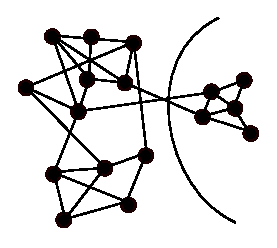
\includegraphics[scale=0.75]{figures/conductance.eps}
\caption{Minimum Conductance Cut attempts to find a sparse cut in the graph.}
\end{figure}
where, for any $S \subseteq V$, the volume $vol(S)$ of $S$ is the sum of the degrees of all the vertices in $S$. The above optimization problem looks for a cut in the graph that simultaneously cuts few edge, while disconnecting a large portion of the graph (where \emph{large} is measured by the volume). The eigenvectors of the Laplacian act as optimizers of the relaxation, and therefore tend to align points in space so as to keep connected points close to each other, while still find inducing meaningful separation among the datapoints. Note that eigenvectors of the normalized Laplacian are solutions to the generalized eigenvalue problem:
\[
    \underset{x \in \mathbb{R}^n}{\text{minimize}}\hspace{1.5mm}{x^TLx \over x^TDx}
\]
or alternatively:
\[
    L\mathbf{x} = \lambda D\mathbf{x}
\]
where $L$ is the (non-normalized) Laplacian matrix: $L = D-A$ and $D$ is defined as above. Spectral embeddings based on the Laplacian are common primitives used in other methods, such as manifold learning, (see for instance (\cite{belkin2003laplacian})). These techniques are also at the heart of a common graph clustering algorithm known as spectral clustering (\cite{ng2002spectral}).
